\subsection{\asf}

\asf\footnote{\url{http://www.symfony-project.org/}} est le \afm\ \aphp\ dont l'initiateur est \apotencier, un des co-fondateurs de \asl. Dans un premier temps conservé en interne dans l'agence, il a finalement été distribué sous licence libre en octobre~2005. Depuis, une véritable communauté internationale s'est formée autour de cet outil. Au delà des qualités techniques intrinsèques de \asf, on peut expliquer ce phénomène par le fait que qu'un effort considérable a été fourni concernant l'écriture de documentation : d'abord rédigée en anglais, elle a ensuite été traduite en plusieurs langues. De plus, plusieurs livres techniques\footnote{Références bibliographiques : \cite{practicalsf} \cite{sfrefguide} \cite{cahierssf} \cite{moresf} \cite{thebook}} ont déjà été publiés, dont la plupart voient leur contenu accessible librement et de façon officielle sur \ainternet.

Les parties suivantes abordent successivement une présentation du concept de \afm, du modèle \amvc, qui est utilisé de manière globale dans \asf, et enfin une énumération des différentes fonctionnalités de \asf.


\subsubsection{Le concept de \afm}

Un \afm\ est comparable à un squelette de programme, à compléter pour mettre en œuvre une application logicielle de façon partielle ou même dans sa totalité. Basé sur les principes de la programmation orientée objet, il se présente sous forme d'un ensemble de classes, abstraites pour les plus importantes, qui prédéfinissent une architecture du programme à réaliser. Associé à cette architecture prédéfinie, un schéma de contrôle d'exécution de programme est également spécifié par les classes.

Les \afms\ ont l'avantage de faciliter le développer d'extensions, la factorisation de fonctionnalités communes, ou encore de favoriser l'interopérabilité des composants. Ils ajoutent des mécanismes nouveaux au-dessus d'un langage de programmation qui rendent le développement plus simple et plus fiable, assemblant des actions complexes dans des actions simplifiées. En outre, ils ajoutent aussi une ligne directrice à la structuration du code qui, connue par un grand nombre de développeurs, améliore de manière drastique la maintenance de l'application.

Toutefois, on peut reprocher aux \afms\ de nécessiter un apprentissage supplémentaire au développeur qui n'est pas toujours évident. Il faut garder à l'esprit que de tels outils, même structurants, peuvent toujours être mal utilisés et donc perdre de leur plus-value. Malgré ces arguments, l'émergence des \afms\ reste sans conteste considéré par l'ensemble des professionnels de l'informatique comme une avancée majeure.

Par ailleurs, l'utilisation de \afms\ dans le contexte du développement web est une approche relativement récente. En effet, pendant longtemps, les sites web ont été plutôt considérés comme des réalisations éphémères ne nécessitant ni une modélisation poussée ni une démarche de qualité et de maintenance. Parallèlement, la façon de développer une application web est en apparence assez exotique : il faut manipuler des entités spécifiques comme la session utilisateur, la requête et la réponse, la persistance des données (souvent effectuée via des requêtes à une base de données) est originale, et l'approche objet est moins évidente. Aussi, le retard dans l'utilisation de \afms\ web est amplifié par le fait que le développement web a pu capter une part importante de programmeurs amateurs qui, n'ayant pas suivi de véritable formation en informatique, ne sont pas au fait des méthodes du génie logiciel.

Le développement massif et toujours croissant d'\ainternet\ oblige les différents acteurs du marché de se positionner sur ce secteur. Ce phénomène est d'autant plus accentué par l'émergence récente et populaire du web~2.0\cite{webdeux} dit \emph{social} ou encore du \acloud\cite{cloud}. Plus que de simples pages, les applications web deviennent alors des systèmes d'information à part entière. Ainsi, aujourd'hui, on ressent vraiment le besoin de faire appel aux différentes méthodes du génie logiciel dans le domaine du développement web, et l'utilisation de \afm\ fait partie intégrante de l'ensemble des solutions.


\subsubsection{Le modèle \amvc}

L'utilisation du \asf\ incite fortement le développeur à respecter les bonnes pratiques du développement web. En effet, toute l'organisation du \afm\ se base sur le patron de conception\footnote{En informatique, un patron de conception est un concept de génie logiciel destiné à résoudre les problèmes récurrents suivant le paradigme objet.\cite{designpattern}} Modèle-Vue-Contrôleur, plus connu sous l'acronyme \amvc. Le but de celui-ci est de séparer complètement les données et les
règles qui les gèrent de leur présentation. Il est alors possible de présenter les mêmes objets, comme par exemple une liste d'actualités, à la fois sous la forme d'une page classique (en \ahtml) et de flux de syndication (aux formats \arss\ et \aatom), le tout sans changer le code concernant la logique de récupération et d'organisation des données.

Pour que cette séparation soit possible, les objets stockés via la couche du modèle ne peuvent pas être conscients de la façon dont ils seront présentés. C'est la couche de la vue qui se chargera de les afficher. En outre, la vue ne présente que des données préparées à l'avance : c'est le contrôleur qui est chargé de récupérer les valeurs adéquates depuis la couche du modèle pour ensuite les transmettre à la vue. L'approche est illustrée dans la figure~\ref{figure:outils_sf_mvc}.

\begin{figure}
	\centering
	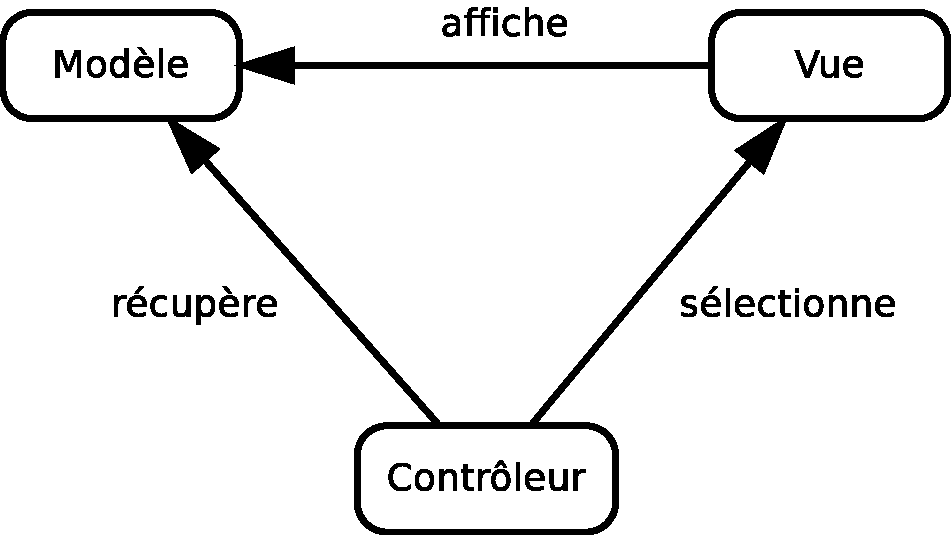
\includegraphics[scale=0.4]{outils_sf_mvc}
	\caption{Interactions entre les trois niveaux du patron de conception \amvc}
	\label{figure:outils_sf_mvc}
\end{figure}

Plus précisément, les trois paragraphes suivants décrivent comment les trois niveaux du \amvc\ s'organisent dans \asf.

\paragraph{Le modèle}

Il représente le comportement de l'application : traitements des données, interactions avec la base de données, etc. Il décrit les données manipulées par l'application et définit les méthodes d'accès. Son implémentation est fortement liée à l'\aorm\ utilisé.\footnote{Cf. section~\ref{section:outils_doctrine} concertant l'\aorm\ \adoctrine}

\paragraph{La vue}

Elle correspond à l'interface avec laquelle l'utilisateur interagit. Plusieurs vues peuvent afficher les informations d'un même modèle, et une même vue peut présenter plusieurs modèles. Via des fichiers appelés \atemplates, elle peut être conçue en \ahtml\ ou tout autre \og langage \fg\ de pré\-sen\-ta\-ti\-on. Elle n'effectue aucun traitement, se contentant d'afficher les résultats de ceux effectués par le modèle.

\paragraph{Le contrôleur}

Il prend en charge la gestion des événements de synchronisation pour mettre à jour la vue ou le modèle. Il n'effectue aucun traitement, ne modifie aucune donnée. Il analyse la requête du client, se contente d'appeler le modèle adéquat et de renvoyer la vue correspondant à la demande. Dans \asf, chaque requête voit sa logique localisée dans ce que l'on appelle une \og action \fg. Elle est accessible via une \og route \fg, qui correspond à l'adresse saisie par l'utilisateur dans son navigateur web.


\subsubsection{Fonctionnalités de \asf}

TODO
